\documentclass{beamer}
\usepackage{listings}
\lstset{
%language=C,
frame=single, 
breaklines=true,
columns=fullflexible
}
\usepackage{subcaption}
\usepackage{url}
\usepackage{tikz}
\usepackage{tkz-euclide} % loads  TikZ and tkz-base
%\usetkzobj{all}
\usetikzlibrary{calc,math}
\usepackage{float}
\newcommand\norm[1]{\left\lVert#1\right\rVert}
\renewcommand{\vec}[1]{\mathbf{#1}}
\usepackage[export]{adjustbox}
\usepackage[utf8]{inputenc}
\usepackage{amsmath}
\usetheme{Boadilla}
\providecommand{\pr}[1]{\ensuremath{\Pr\left(#1\right)}}
\providecommand{\sbrak}[1]{\ensuremath{{}\left[#1\right]}}
\providecommand{\lsbrak}[1]{\ensuremath{{}\left[#1\right.}}
\providecommand{\rsbrak}[1]{\ensuremath{{}\left.#1\right]}}
\providecommand{\brak}[1]{\ensuremath{\left(#1\right)}}
\providecommand{\lbrak}[1]{\ensuremath{\left(#1\right.}}
\providecommand{\rbrak}[1]{\ensuremath{\left.#1\right)}}
\providecommand{\cbrak}[1]{\ensuremath{\left\{#1\right\}}}
\providecommand{\lcbrak}[1]{\ensuremath{\left\{#1\right.}}
\providecommand{\rcbrak}[1]{\ensuremath{\left.#1\right\}}}

\title{Research paper presentation}
\author{N.Manaswini-CS20BTECH11035}
\date{}
\begin{document}

\begin{frame}
\titlepage
\end{frame}

\begin{frame}
\begin{block}{Title}
Performance Analysis of NOMA Assisted Underwater Visible
Light Communication System
\end{block}
\begin{block}{Authors}
\begin{enumerate}
\item Monika Jain
\item Nikhil Sharma, Member, IEEE
\item Akash Gupta , Member, IEEE
\item Divyang Rawal, Member, IEEE
\item Parul Garg , Senior Member, IEEE
\end{enumerate}
\end{block}
\end{frame}





\begin{frame}
\begin{block}{Prerequisites}
\begin{enumerate}
\item Meijer g function
\item fox H function
\item NOMA
\item error function and complementary error function
\end{enumerate}
\end{block}
\begin{block}{Non Orthogonal Multiple Access(NOMA)}
NOMA was proposed as a candidate radio access technology for 5G cellular systems.Non-orthogonal multiple access (NOMA) has evolved as a spectrally efficient,multiple access scheme that can cater to a large number of devices.This presentation presents analytical investigation of NOMA assisted Underwater Visible Light Communication(UWVLC) system.
\end{block}
\end{frame}


\begin{frame}
\begin{block}{Meijer G function}
It is defined as follows:
\begin{align}
G^{m,n}_{p,q} \sbrak{\begin{array}{c}
a_1,..,a_p \\
b_1,..,b_q 
\end{array} \middle \vert
\begin{array}{c}
z
\end{array} } &= \frac{1}{2 \pi \mathfrak{i}} \int_L \frac{\Pi_{j=1}^m \Gamma(b_j-s)\Pi_{j=1}^n \Gamma(1-a_j+s)}{\Pi_{j=m+1}^q \Gamma(1-b_j+s)\Pi_{j=n+1}^p \Gamma(a_j-s)} z^s \mathrm{d}s \label{g}
\end{align}
where,
\begin{enumerate}
\item $\Gamma()$ is gamma function
\item $0 \leq m \leq q$,$0 \leq n \leq p$ and m,n,p,q are integers
\item $a_k-b_j \neq 1,2,3...$ for $k=1,2,....,n$,$j=1,2,....,m$
\item $z \neq 0$
\end{enumerate}
\end{block}
\end{frame}




\begin{frame}
\begin{block}{Fox H function}
It is defined as follows:
\begin{align}
H^{m,n}_{p,q} & \sbrak{\begin{array}{c}
z
\end{array} \middle \vert
\begin{array}{c}
(a_1,A_1),..,(a_p,A_p) \\
(b_1,B_1),..,(b_q,B_q) 
\end{array} }   \notag \\ 
 &= \frac{1}{2 \pi \mathfrak{i}} \int_L \frac{\Pi_{j=1}^m \Gamma(b_j+B_js)\Pi_{j=1}^n \Gamma(1-a_j-A_js)}{\Pi_{j=m+1}^q \Gamma(1-b_j-B_js)\Pi_{j=n+1}^p \Gamma(a_j+A_js)} z^{-s} \mathrm{d}s \label{f}
\end{align}
\end{block}
\begin{block}{Error function(erf) and complementary error function(erfc)}
\begin{align}
erf(z) &= \frac{2}{\sqrt{\pi}} \int_0^z e^{-t^2} \mathrm{d}t \label{erf} \\
erfc(z) &= 1- erf(z) \label{erfc}
\end{align}
\end{block}
\end{frame}



\begin{frame}
\begin{block}{NOMA users}
The system model of NOMA UWVLC consists of the
underwater NOMA users, i.e., near-user UV1 and far user
(UV2) at different height or distance from the on-surface
floating vehicle (FV).
\end{block}
\begin{block}{Transmitted superposition coded signal(${\hat{r}}_{sc}$)}
\begin{align}
{\hat{r}}_{sc}=\sqrt{\psi_1}s_1 + \sqrt{\psi_2}s_2 \label{rsc}
\end{align}
where,\\
\begin{enumerate}
\item $\psi_1=\delta P_t$ is the ratio of power allocated to $UV_1$
\item $\psi_2=(1-\delta) P_t$ is the ratio of power allocated to $UV_2$
\item $\delta$ is the Power Allocation Coefficient
\item $P_t$ is the power transmitted by the source
\item $s_1,s_2$ are on-off keying (OOK) modulated symbols for users $UV_1$
and $UV_2$ respectively.
\end{enumerate}
\end{block}
\end{frame}


\begin{frame}
\frametitle{Received signal}
FV(Floating vehicle) transmits this signal to NOMA users($UV_1$,$UV_1$) as $FV-UV_1$,$FV-UV_2$ respectively(assumed to be EGG (Exponential generalised gamma) distributed.
\begin{block}{Received signal}
\begin{align}
y_{UV_i} = \eta I_i \hat{r}_sc +n_i  \label{yuv}
\end{align}
where,\\
\begin{enumerate}
\item $i=1,2$
\item $\eta$ is responsivity(optical to electrical conversion coefficient)
\item $I_i$ is real valued irradiance fluctuation.
\item $n_i$ is the Additive White Gaussian Noice(AWGN) $ \sim \mathcal{N}(0,\frac{N_0}{2})$
\item ${\hat{r}}_{sc}$ is transmitted Super coded signal
\end{enumerate}
\end{block}
\end{frame}





\begin{frame}
\begin{block}{PDF of UWVLC channel}
\begin{align}
f_{\rho}(\rho)=\frac{w_0}{r \rho}G^{1,0}_{0,1} \sbrak{\begin{array}{c}
\frac{1}{{\lambda}_0}\brak{\frac{\rho}{{\mu}_r}}^\frac{1}{r}  
\end{array} \middle \vert
\begin{array}{c}
- \\
1
\end{array} } + \frac{c_0(1-w_0)}{r \rho \Gamma(a_0)}G^{1,0}_{0,1} \sbrak{\begin{array}{c}
\frac{1}{b_0^{c_0}}\brak{\frac{\rho}{{\mu}_r}}^\frac{c_0}{r}  
\end{array} \middle \vert
\begin{array}{c}
- \\
a_0
\end{array} } \label{pdf}
\end{align}
where,
\begin{enumerate}
\item $\rho=\frac{(\eta I)^r}{N_0}$
\item $N_0$ is noise power
\item r depicts detection technique involved
\begin{enumerate}
\item  $r=1$ represents heterodyne detection(HD)
\item  $r=2$ represents intensity modulation/direct detection (IM/DD)
\end{enumerate}
\item $w_0$ is mixture coefficient of GG(generalized gamma) distribution
\item $\lambda_0$ is scale parameter of Exponential distribution
\item $a_0,b_0,c_0$ are parameters of GG(generalized gamma) distribution
\item $\mu_r$ is function of average electrical SNR(signal to noise ratio)
\item $G,\Gamma()$ are meijer g function,gamma function respectively
\end{enumerate}
\end{block}
\end{frame}





\begin{frame}
\textbf{signal constellation of NOMA far user $UV_2$} \\
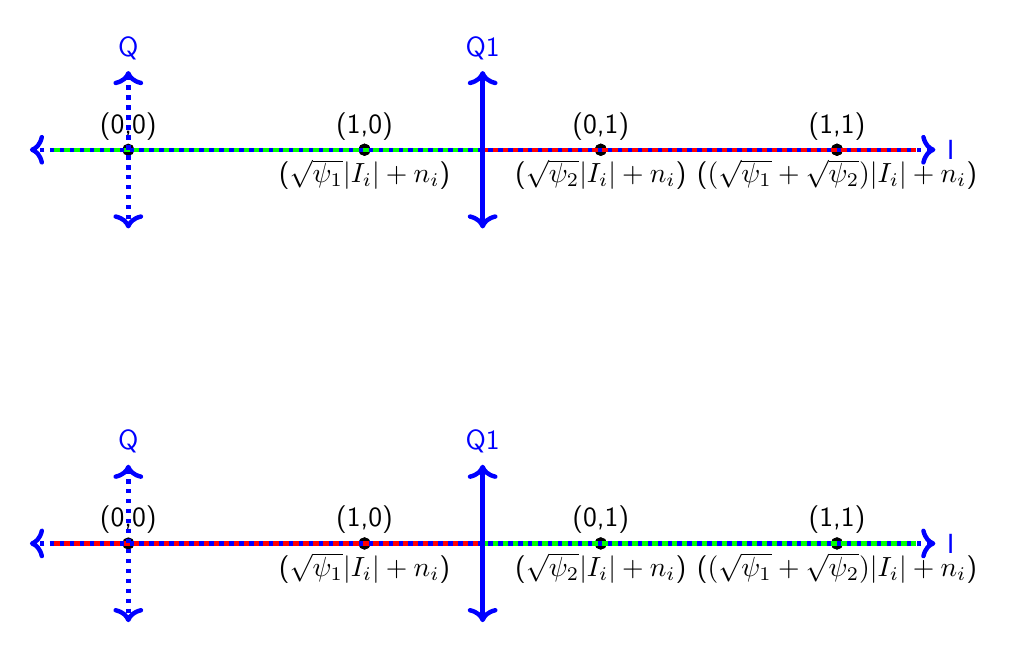
\begin{tikzpicture}[font=\sffamily]


   \tikzset{node style/.style={circle,
                               draw=blue!10, 
                               fill=blue!10,
                               ultra thick,
                               minimum size=5mm,
                               }}

    \filldraw[black] (0,0) circle(2pt) node[anchor=south] {(0,0)};
    \filldraw[black] (3,0) circle(2pt) node[anchor=south] {(1,0)};
    \filldraw[black] (6,0) circle(2pt) node[anchor=south] {(0,1)};
    \filldraw[black] (9,0) circle(2pt) node[anchor=south] {(1,1)};
    
    \filldraw[black] (0,-5) circle(2pt) node[anchor=south] {(0,0)};
    \filldraw[black] (3,-5) circle(2pt) node[anchor=south] {(1,0)};
    \filldraw[black] (6,-5) circle(2pt) node[anchor=south] {(0,1)};
    \filldraw[black] (9,-5) circle(2pt) node[anchor=south] {(1,1)};
    
    
    
    \filldraw[black] (3,0) circle(2pt) node[anchor=north] {($\sqrt{\psi_1}    
|I_i|+n_i$)};
    \filldraw[black] (6,0) circle(2pt) node[anchor=north] {($\sqrt{\psi_2}    
|I_i|+n_i$)};
    \filldraw[black] (9,0) circle(2pt) node[anchor=north] {($(\sqrt{\psi_1}    + \sqrt{\psi_2})|I_i|+n_i$)};
    

    \filldraw[black] (3,-5) circle(2pt) node[anchor=north] {($\sqrt{\psi_1}    
|I_i|+n_i$)};
    \filldraw[black] (6,-5) circle(2pt) node[anchor=north] {($\sqrt{\psi_2}    
|I_i|+n_i$)};
    \filldraw[black] (9,-5) circle(2pt) node[anchor=north] {($(\sqrt{\psi_1}    + \sqrt{\psi_2})|I_i|+n_i$)};    
    
    

    \draw[green,ultra thick] (-1,0) -- (4.5,0);
    \draw[red,ultra thick] (4.5,0) -- (10,0);  
    \draw[<->,blue,dotted,ultra thick] (0,1) -- (0,-1)  node[pos=0,above] {Q}  ; 
    \draw[<->,blue,ultra thick] (4.5,1) -- (4.5,-1) node[pos=0,above] {Q1};
    \draw[<->,blue,dotted,ultra thick] (10.25,0) --  (-1.25,0) node[pos=0,right] {I}  ; 
    
    
    
    
    \draw[red,ultra thick] (-1,-5) -- (4.5,-5);
    \draw[green,ultra thick] (4.5,-5) -- (10,-5);  
    \draw[<->,blue,dotted,ultra thick] (0,-4) -- (0,-6)  node[pos=0,above] {Q}  ; 
    \draw[<->,blue,ultra thick] (4.5,-4) -- (4.5,-6) node[pos=0,above] {Q1};
    \draw[<->,blue,dotted,ultra thick] (10.25,-5) --  (-1.25,-5) node[pos=0,right] {I}  ;
    \end{tikzpicture} 

\end{frame}








\begin{frame}
\textbf{signal constellation of NOMA near user $UV_1$} \\
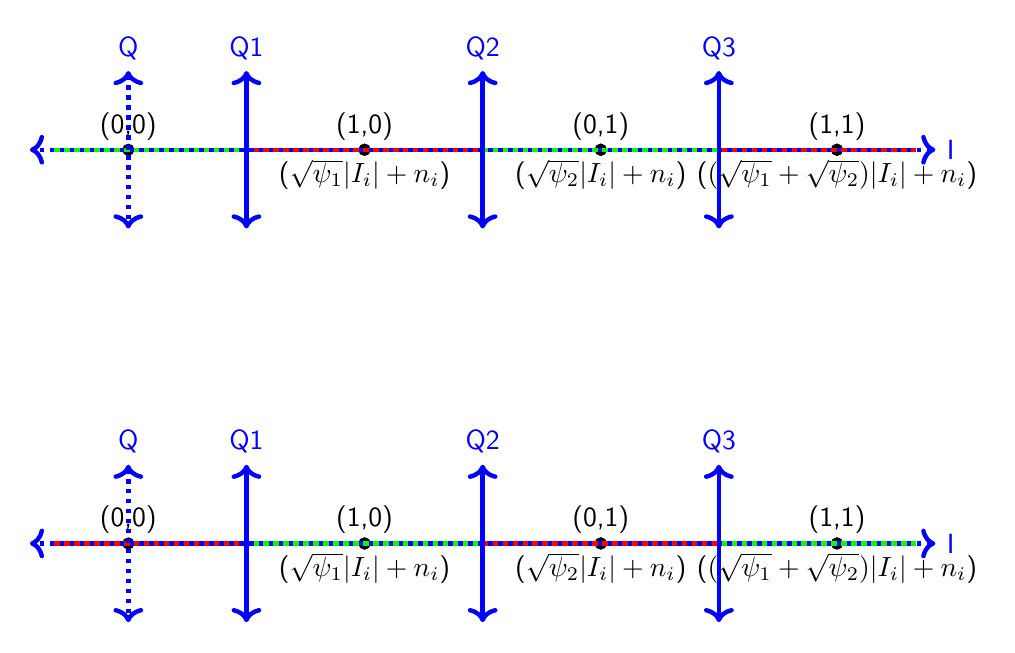
\begin{tikzpicture}[font=\sffamily]


   \tikzset{node style/.style={rectangle,
                               draw=blue!10, 
                               fill=blue!10,
                               ultra thick,
                               minimum size=5mm,
                               }}

    \filldraw[black] (0,0) circle(2pt) node[anchor=south] {(0,0)};
    \filldraw[black] (3,0) circle(2pt) node[anchor=south] {(1,0)};
    \filldraw[black] (6,0) circle(2pt) node[anchor=south] {(0,1)};
    \filldraw[black] (9,0) circle(2pt) node[anchor=south] {(1,1)};
    
    \filldraw[black] (0,-5) circle(2pt) node[anchor=south] {(0,0)};
    \filldraw[black] (3,-5) circle(2pt) node[anchor=south] {(1,0)};
    \filldraw[black] (6,-5) circle(2pt) node[anchor=south] {(0,1)};
    \filldraw[black] (9,-5) circle(2pt) node[anchor=south] {(1,1)};
    
    
    
    
    \filldraw[black] (3,0) circle(2pt) node[anchor=north] {($\sqrt{\psi_1}    
|I_i|+n_i$)};
    \filldraw[black] (6,0) circle(2pt) node[anchor=north] {($\sqrt{\psi_2}    
|I_i|+n_i$)};
    \filldraw[black] (9,0) circle(2pt) node[anchor=north] {($(\sqrt{\psi_1}    + \sqrt{\psi_2})|I_i|+n_i$)};
    

    \filldraw[black] (3,-5) circle(2pt) node[anchor=north] {($\sqrt{\psi_1}    
|I_i|+n_i$)};
    \filldraw[black] (6,-5) circle(2pt) node[anchor=north] {($\sqrt{\psi_2}    
|I_i|+n_i$)};
    \filldraw[black] (9,-5) circle(2pt) node[anchor=north] {($(\sqrt{\psi_1}    + \sqrt{\psi_2})|I_i|+n_i$)};    
    
    
    
    

    \draw[green,ultra thick] (-1,0) -- (1.5,0);
    \draw[red,ultra thick] (1.5,0) -- (4.5,0);  
    \draw[green,ultra thick] (4.5,0) -- (7.5,0);
    \draw[red,ultra thick] (7.5,0) -- (10,0); 
    \draw[<->,blue,dotted,ultra thick] (0,1) -- (0,-1)  node[pos=0,above] {Q}  ; 
    \draw[<->,blue,ultra thick] (4.5,1) -- (4.5,-1) node[pos=0,above] {Q2};
    \draw[<->,blue,ultra thick] (1.5,1) -- (1.5,-1)  node[pos=0,above] {Q1}  ; 
    \draw[<->,blue,ultra thick] (7.5,1) -- (7.5,-1) node[pos=0,above] {Q3};
    \draw[<->,blue,dotted,ultra thick] (10.25,0) --  (-1.25,0) node[pos=0,right] {I}  ; 
    
    
    
    
    \draw[red,ultra thick] (-1,-5) -- (1.5,-5);
    \draw[green,ultra thick] (1.5,-5) -- (4.5,-5);  
    \draw[red,ultra thick] (4.5,-5) -- (7.5,-5);
    \draw[green,ultra thick] (7.5,-5) -- (10,-5); 
    \draw[<->,blue,dotted,ultra thick] (0,-4) -- (0,-6)  node[pos=0,above] {Q}  ; 
    \draw[<->,blue,ultra thick] (4.5,-4) -- (4.5,-6) node[pos=0,above] {Q2};
    \draw[<->,blue,ultra thick] (1.5,-4) -- (1.5,-6)  node[pos=0,above] {Q1}  ; 
    \draw[<->,blue,ultra thick] (7.5,-4) -- (7.5,-6) node[pos=0,above] {Q3};
    \draw[<->,blue,dotted,ultra thick] (10.25,-5) --  (-1.25,-5) node[pos=0,right] {I}  ;
    \end{tikzpicture} 

\end{frame}




\begin{frame}
\frametitle{Average BER}
\begin{block}{Bit error rate}
BER(Bit error rate) is the number of bit errors per unit time.These errors may occur due to noise, interference , distortion etc
\end{block}
\begin{block}{Instantaneous BER of far user $UV_2$}
The bit $s2 = 0$ of symbol $(0, 0)$ and $(1, 0)$ is erroneously detected as $s2 = 1$ 
The PDF of constellation point $(0, 0)$ can be expressed as 
\begin{align}
f_{0,0}&=\frac{1}{\sqrt{2 \pi \sigma^2}}e^{-\frac{(x-0)^2}{2 \sigma^2}}
\end{align}
The error probability of point (0, 0) is($\sigma^2=\frac{N_0}{2}$)
\begin{align}
P_{{UV_2}_{|(0,0)}} &= \frac{1}{4} \int_{\sqrt{\frac{{\rho_1}}{2}}}^\infty e^{-\frac{(x-0)^2}{N_0^2}} \mathrm{d}x  =  \frac{1}{4}  Q(\sqrt{\rho_1})
\end{align}
\end{block}
\end{frame}



\begin{frame}
\frametitle{Average BER}
\begin{block}{Instantaneous BER of far user $UV_2$}
Similarly,
\begin{align}
P_{{UV_2}_{|(1,0)}} &=  \frac{1}{4} \int_{\sqrt{\frac{{\rho_2}}{2}}}^\infty e^{-\frac{x^2}{N_0^2}} \mathrm{d}x  =  \frac{1}{4} Q(\sqrt{\rho_2})\\
P_{{UV_2}_{|(0,1)}} &= \frac{1}{4}  \int_{\sqrt{\frac{{\rho_2}}{2}}}^\infty e^{-\frac{x^2}{N_0^2}} \mathrm{d}x - \frac{1}{4} \int_{\sqrt{\frac{{\rho_3}}{2}}}^\infty e^{-\frac{x^2}{N_0^2}} \mathrm{d}x = \frac{1}{4} \brak{ Q(\sqrt{\rho_2})-Q(\sqrt{\rho_3})} \\
P_{{UV_2}_{|(1,1)}} &=  \frac{1}{4} \int_{\sqrt{\frac{{\rho_1}}{2}}}^\infty e^{-\frac{x^2}{N_0^2}} \mathrm{d}x - \frac{1}{4} \int_{\sqrt{\frac{{\rho_4}}{2}}}^\infty e^{-\frac{x^2}{N_0^2}} \mathrm{d}x =  \frac{1}{4} \brak{Q(\sqrt{\rho_1})-Q(\sqrt{\rho_4})}\\
P_{UV_2} &= P_{{UV_2}_{|(0,0)}}+ P_{{UV_2}_{|(1,0)}} + P_{{UV_2}_{|(0,1)}}+P_{{UV_2}_{|(1,1)}}\\
P_{UV_2} &= \frac{1}{4} \brak{2Q(\sqrt{\rho_1})+2Q(\sqrt{\rho_2})-Q(\sqrt{\rho_3})-Q(\sqrt{\rho_4})} \label{puv2}
\end{align}
\end{block}
\end{frame}


\begin{frame}
\frametitle{Average BER}
\begin{block}{Instantaneous BER of far user $UV_2$}
where,
\begin{enumerate}
\item  Q(.) denotes Q-function
\item  $\rho_1= \frac{(\sqrt{\psi_1}+\sqrt{\psi_2})^2|I_2|^2}{2N_0}$
\item  $\rho_2= \frac{(\sqrt{\psi_2}-\sqrt{\psi_1})^2|I_2|^2}{2N_0}$
\item  $\rho_3= \frac{2\psi_2|I_2|^2}{N_0}$
\item  $\rho_4= \frac{2(\sqrt{\psi_1}+\sqrt{\psi_2})^2|I_2|^2}{N_0}$
\end{enumerate}
\end{block}
\end{frame}

\begin{frame}
\begin{block}{Instantaneous BER of near user $UV_1$}
\begin{align}
P_{{UV_1}_{|(0,0) \rightarrow (1,0)}} &= \frac{1}{4} \brak{ Q(\sqrt{\rho_6})-Q(\sqrt{\rho_{12}})}\\
P_{{UV_1}_{|(0,0) \rightarrow (1,1)}} &=\frac{1}{4}  Q(\sqrt{\rho_{10}}) \\
P_{{UV_1}_{|0,1) \rightarrow (1,0)}} &=  \frac{1}{4} \brak{Q(\sqrt{\rho_8})-Q(\sqrt{\rho_9})}\\
P_{{UV_1}_{|(0,1) \rightarrow (1,1)}} &= \frac{1}{4}  Q(\sqrt{\rho_6}) \\
P_{{UV_1}_{|(1,0) \rightarrow (0,0)}} &= \frac{1}{4} \brak{Q(\sqrt{\rho_5})-Q(\sqrt{\rho_7})}\\
P_{{UV_1}_{|(1,0) \rightarrow (0,1)}} &= \frac{1}{4} \brak{Q(\sqrt{\rho_8})-Q(\sqrt{\rho_9})}\\
P_{{UV_1}_{|(1,1) \rightarrow (0,1)}} &=\frac{1}{4} \brak{ Q(\sqrt{\rho_6})-Q(\sqrt{\rho_{12}})}\\
P_{{UV_1}_{|(1,1) \rightarrow (0,0)}} &=\frac{1}{4} \brak{ Q(\sqrt{\rho_{12}})-Q(\sqrt{\rho_{11}})} 
\end{align}
\end{block}
\end{frame}



\begin{frame}
\frametitle{Average BER}
\begin{block}{Instantaneous BER of near user $UV_1$}
\begin{align}
P_{UV_1} &= P_{{UV_1}_{|(0,0) \rightarrow (1,0)}} +P_{{UV_1}_{|(0,0) \rightarrow (1,1)}} +P_{{UV_1}_{|0,1) \rightarrow (1,0)}} \notag  \\  &+P_{{UV_1}_{|0,1) \rightarrow (1,1)}} + P_{{UV_1}_{|(1,0) \rightarrow (0,0)}} +P_{{UV_1}_{|(1,0) \rightarrow (0,1)}} \notag  \\ & + P_{{UV_1}_{|(1,1) \rightarrow (0,1)}} + P_{{UV_1}_{|(1,1) \rightarrow (0,0)}} \\
P_{UV_1} &= \frac{1}{4} \brak{Q(\sqrt{\rho_5})+3Q(\sqrt{\rho_6})-Q(\sqrt{\rho_7})+2Q(\sqrt{\rho_8})-2Q(\sqrt{\rho_9})} \notag \\ 
 &+\frac{1}{4} \brak{Q(\sqrt{\rho_{10}})-Q(\sqrt{\rho_{11}})-Q(\sqrt{\rho_{12}})} \label{puv1}
\end{align}
\end{block}
\end{frame}

\begin{frame}
\frametitle{Average BER}
\begin{block}{Instantaneous BER of far user $UV_1$}
where,
\begin{enumerate}
\item  Q(.) denotes Q-function
\item  $\rho_5= \frac{(\sqrt{\psi_1}-\sqrt{\psi_2})^2|I_1|^2}{2N_0}$
\item  $\rho_6= \frac{\psi_1|I_1|^2}{2N_0}$
\item  $\rho_7= \frac{2\psi_1|I_1|^2}{N_0}$
\item  $\rho_8= \frac{(\sqrt{\psi_2}-\sqrt{\psi_1})^2|I_1|^2}{2N_0}$
\item  $\rho_9= \frac{(2\sqrt{\psi_2}-\sqrt{\psi_1})^2|I_1|^2}{2N_0}$
\item  $\rho_{10}= \frac{(2\sqrt{\psi_2}+\sqrt{\psi_1})^2|I_1|^2}{2N_0}$
\item  $\rho_{11}= \frac{2(\sqrt{\psi_2}-\sqrt{\psi_1})^2|I_1|^2}{2N_0}$
\item  $\rho_{12}= \frac{(\sqrt{\psi_1}+\sqrt{\psi_2})^2|I_1|^2}{2N_0}$
\end{enumerate}
\end{block}
\end{frame}


\begin{frame}
\frametitle{Average BER}
\begin{block}{Average BER}
\begin{align}
\bar{P}_{UV_i} &= \int_0^\infty P_{UV_i}f_{\rho}(\rho) \mathrm{d}\rho \label{avgb} \\
Q(x) &= \frac{1}{2}erfc(\frac{x}{\sqrt{2}}) \label{qerfc} \\
erfc(\sqrt{x}) &= \frac{1}{\sqrt{\pi}} G^{2,0}_{1,2} \sbrak{\begin{array}{c}
x 
\end{array} \middle \vert
\begin{array}{c}
1 \\
0,\frac{1}{2}
\end{array} } \label{gerfc}
\end{align}
Average BER can be obtained by using \eqref{puv1},\eqref{puv2},\eqref{pdf},\eqref{gerfc},\eqref{qerfc},we get
\begin{align}
\bar{P}_{UV_1} &= \frac{1}{4} \brak{ X(\bar{\rho_5}) +3 X(\bar{\rho_6}) - X(\bar{\rho_7}) +2 X(\bar{\rho_8}) -2 X(\bar{\rho_9}) } \notag \\
&+\frac{1}{4} \brak{  X(\bar{\rho_{10}}) - X(\bar{\rho_{11}})- X(\bar{\rho_{12}})}  \label{apuv1} \\
\bar{P}_{UV_2} &= \frac{1}{4} \brak{ 2X(\bar{\rho_1}) + 2 X(\bar{\rho_2})- X(\bar{\rho_3})-  X(\bar{\rho_4})} \label{apuv2}
\end{align}
\end{block}
\end{frame}



\begin{frame}
\frametitle{Average BER}
\begin{block}{Average BER}
where,
\begin{enumerate}
\item $\bar{\rho_j} = E(\rho_j)$ where $j=1,2,3,4$ for NOMA far user($UV_2$) ,$j=5,6,7,...12$ for NOMA near user($UV_1$)  
\item $\mu_r=\frac{\bar{\rho_j}}{2w_0 \lambda_0^2 +b_0^2(1-w_0) \frac{\Gamma(a_0+\frac{2}{c_0})}{\Gamma(a_0)}}$
\item \begin{align}
X(\bar{\rho_j}) = \frac{w_0}{2 \sqrt{\pi}}H^{1,2}_{2,2} & \sbrak{\begin{array}{c}
\frac{2}{\lambda_0^r \mu_r}
\end{array} \middle \vert
\begin{array}{c}
(1,1),(\frac{1}{2},1) \\
(1,r),(0,1) 
\end{array} }  + \notag \\ 
& \frac{(1-w_0)}{2 \sqrt{\pi} \Gamma(a_0)} H^{1,2}_{2,2} \sbrak{\begin{array}{c}
\frac{2}{b_0^r \mu_r}
\end{array} \middle \vert
\begin{array}{c}
(1,1),(\frac{1}{2},1) \\
(a_0,\frac{r}{c_0}),(0,1) 
\end{array} } 
\end{align}
\item $r=2$ 
\end{enumerate}
\end{block}
\end{frame}


\begin{frame}
\frametitle{Average BER graphs}
\begin{figure}[htb!]
\begin{center}
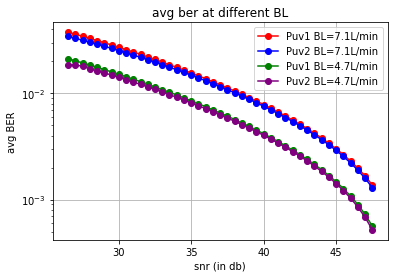
\includegraphics[width=0.48\columnwidth]{BL.png}
\end{center}
\end{figure}

\begin{figure}[htb!]
\begin{center}
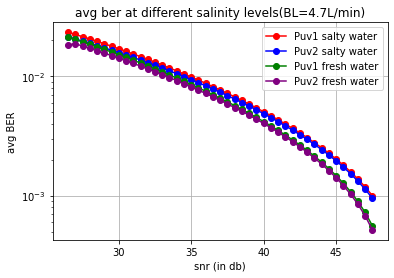
\includegraphics[width=0.48\columnwidth]{salinitylevel.png}
\end{center}
\end{figure}
\end{frame}

\begin{frame}
\frametitle{Average BER graphs}
\begin{figure}[htb!]
\begin{center}
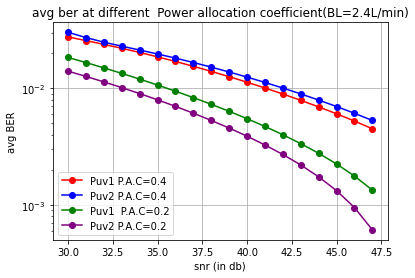
\includegraphics[width=0.48\columnwidth]{PAC.png}
\end{center}
\end{figure}

\begin{figure}[htb!]
\begin{center}
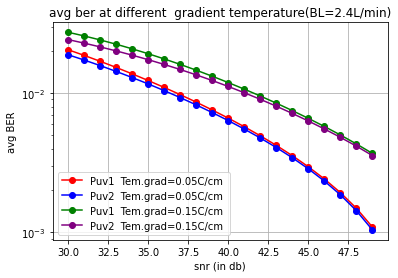
\includegraphics[width=0.48\columnwidth]{gradtemp.png}
\end{center}
\end{figure}
\end{frame}







\begin{frame}
\frametitle{Ergodic Capacity}
\begin{block}{Ergodic Capacity}
Sum rate of NOMA UWVLC (Ergodic Capacity) is given as
\begin{align}
C_{sum} &= \sum_{i=1}^2 C_{UV_i} \label{ec} \\
C_{UV_i} &= E[\ln{(1+\zeta \rho_{UV_i})}] \label{cuvi} \\
\zeta &= \frac{e}{2 \pi}
\end{align}
Solving \eqref{cuvi} we get 
\begin{align}
C_{UV_i}  = {w_0}H^{3,1}_{2,3} & \sbrak{\begin{array}{c}
\frac{1}{\lambda_0^r \zeta \mu_r}
\end{array} \middle \vert
\begin{array}{c}
(0,1),(1,1) \\
(1,r),(0,1) ,(0,1)
\end{array} }  + \notag \\ 
& \frac{(1-w_0)}{\Gamma(a_0)} H^{3,1}_{2,3} \sbrak{\begin{array}{c}
\frac{1}{b_0^r \zeta \mu_r}
\end{array} \middle \vert
\begin{array}{c}
(0,1),(1,1) \\
(a_0,\frac{r}{c_0}),(0,1) ,(0,1) 
\end{array} } 
\end{align}
\end{block}
\end{frame}


\begin{frame}
\frametitle{Ergodic Capacity}
\begin{block}{Ergodic Capacity}
where,
\begin{enumerate}
\item $\bar{\rho}_{UV_1} = \frac{\delta P_t E[|I_1|^2]}{N_0} $  
\item $\bar{\rho}_{UV_2} = \frac{(1-\delta) P_t E[|I_2|^2]}{\delta P_t E[|I_2|^2]+N_0} $ 
\item $\mu_r=\frac{\bar{\rho}_{UV_i}}{2w_0 \lambda_0^2 +b_0^2(1-w_0) \frac{\Gamma(a_0+\frac{2}{c_0})}{\Gamma(a_0)}}$ where $i=1,2$
\item $r=2$ 
\item $\delta$ is power allocation coefficient
\end{enumerate}
\end{block}
\end{frame}


\begin{frame}
\frametitle{Ergodic capacity graphs}
\begin{figure}[htb!]
\begin{center}
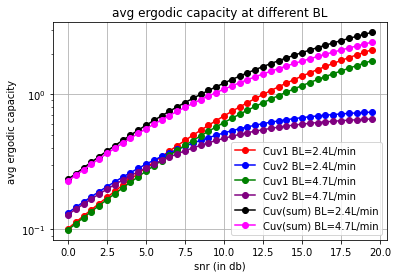
\includegraphics[width=0.48\columnwidth]{ec_BL.png}
\end{center}
\end{figure}

\begin{figure}[htb!]
\begin{center}
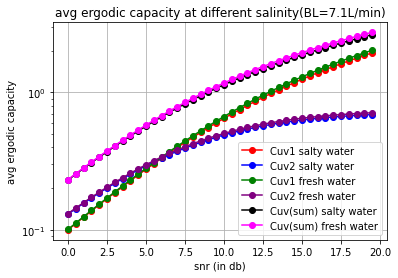
\includegraphics[width=0.48\columnwidth]{ec_sal.png}
\end{center}
\end{figure}
\end{frame}

\begin{frame}
\frametitle{Ergodic capacity graphs}
\begin{figure}[htb!]
\begin{center}
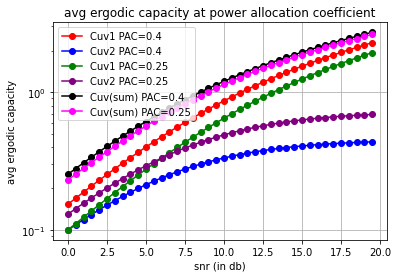
\includegraphics[width=0.48\columnwidth]{ec_PAC.png}
\end{center}
\end{figure}

\begin{figure}[htb!]
\begin{center}
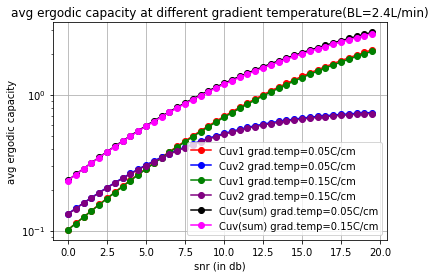
\includegraphics[width=0.48\columnwidth]{ec_gradtemp.png}
\end{center}
\end{figure}
\end{frame}




\end{document}